
%{{第五十三回}}{第五十三回}}

\chapter{宁国府除夕祭宗祠\hspace{.5em}荣国府元宵开夜宴}

{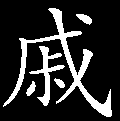
\includegraphics[width=3mm]{../Images/00005}  \kaishu “除夕祭宗祠”一题极博大,“元宵开夜宴”一题极富丽,拟此二题于一回中,早令人惊心动魄。不知措手处,乃作者偏就宝琴眼中款款叙来。首叙院宇匾对,次叙抱厦匾对,后叙正堂匾对,字字古艳。槛以外,槛以内,是男女分界处;仪门以外,仪门以内,是主仆分界处。献帛献爵择其人,应昭应穆从其讳,是一篇绝大典制文字。最高妙是神主“看不真切”一句,最苦心是用贾蓉为槛边传蔬人,用贾芷为仪门传蔬人,体贴入细。噫!文心至此,脉绝血枯矣。谁是知音者?}

话说宝玉见晴雯将雀裘补完,已使的力尽神危,忙命小丫头子来替他捶着,彼此捶打了一会歇下。没一顿饭的工夫,天已大亮,且不出门,只叫快传大夫。一时王太医来了,诊了脉,疑惑说道:“昨日已好了些,今日如何反虚浮微缩起来,敢是吃多了饮食?不然就是劳了神思。外感却倒清了,这汗后失于调养,非同小可。一面说,一面出去开了药方进来。宝玉看时,已将疏散驱邪诸药减去了,倒添了茯苓、地黄、当归等益神养血之剂。宝玉忙命人煎去,一面叹说:“这怎么处!倘或有个好歹,都是我的罪孽。”晴雯睡在枕上嗐道:“好太爷!你干你的去罢!那里就得痨病了。”宝玉无奈,只得去了。至下半天,说身上不好就回来了。晴雯此症虽重,幸亏他素习是个使力不使心的;再者素习饮食清淡,饥饱无伤。这贾宅中的风俗秘法,无论上下,只一略有些伤风咳嗽,总以净饿为主,次则服药调养。故于前日一病时,净饿了两三日,又谨慎服药调治,如今劳碌了些,又加倍培养了几日,便渐渐的好了。近日园中姊妹皆各在房中吃饭,炊爨饮食亦便,宝玉自能变法要汤要羹调停,不必细说。

袭人送母殡后,业已回来,麝月便将平儿所说宋妈坠儿一事,并晴雯撵逐出去等话,一一也曾回过宝玉。袭人也没别说,只说太性急了些。只因李纨亦因时气感冒;邢夫人又正害火眼,迎春岫烟皆过去朝夕侍药;{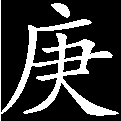
\includegraphics[width=3mm]{../Images/00004}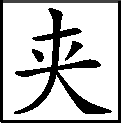
\includegraphics[width=3mm]{../Images/00012}\footnotesize \kaishu 妙在一人不落,事事皆到。}李婶之弟又接了李婶和李纹李绮家去住几日;{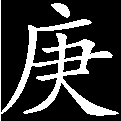
\includegraphics[width=3mm]{../Images/00004}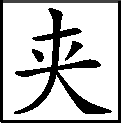
\includegraphics[width=3mm]{../Images/00012}\footnotesize \kaishu 来的也有理,去的也有情。}宝玉又见袭人常常思母含悲,晴雯犹未大愈:因此诗社之日,皆未有人作兴,便空了几社。

当下已是腊月,离年日近,王夫人与凤姐治办年事。王子腾升了九省都检点,贾雨村补授了大司马,协理军机参赞朝政,不题。

且说贾珍那边,开了宗祠,着人打扫,收拾供器,请神主,又打扫上房,以备悬供遗真影像。此时荣宁二府内外上下,皆是忙忙碌碌。这日,宁府中尤氏正起来,同贾蓉之妻打点送贾母这边针线礼物,正值丫头捧了一茶盘押岁锞子进来,回说:“兴儿回奶奶,前儿那一包碎金子共是一百五十三两六钱七分,里头成色不等,共总倾了二百二十个锞子。”说着递上去。尤氏看了看,只见也有梅花式的,也有海棠式的,也有笔锭如意的,也有八宝联春的。尤氏命:“收起这个来,叫他把银锞子快快交了进来。”丫鬟答应去了。

一时贾珍进来吃饭,贾蓉之妻回避了。贾珍因问尤氏:“咱们春祭的恩赏可领了不曾?”尤氏道:“今儿我打发蓉儿关去了。”贾珍道:“咱们家虽不等这几两银子使,多少是皇上天恩。早关了来,给那边老太太见过,置了祖宗的供,上领皇上的恩,下则是托祖宗的福。咱们那怕用一万银子供祖宗,到底不如这个,又体面,又是沾恩锡福的。除咱们这样一二家之外,那些世袭穷官儿家,若不仗着这银子,拿什么上供过年?真正皇恩浩大,想的周到。”尤氏道:“正是这话。”

二人正说着,只见人回:“哥儿来了。”贾珍便命叫他进来。只见贾蓉捧了一个小黄布口袋进来。贾珍道:“怎么去了这一日。”贾蓉陪笑回说:“今儿不在礼部关领,又分在光禄寺库上,因又到了光禄寺才领了下来。光禄寺的官儿们都说问父亲好,多日不见,都着实想念。”贾珍笑道:“他们那里是想我。这又到了年下了,不是想我的东西,就是想我的戏酒了。”一面说,一面瞧那黄布口袋,上有印就是“皇恩永锡”四个大字,那一边又有礼部祠祭司的印记,又写着一行小字,道是“宁国公贾演、荣国公贾源,恩赐永远春祭赏共二分,净折银若干两,某年月日龙禁尉候补侍卫贾蓉当堂领讫,值年寺丞某人”,下面一个朱笔花押。

贾珍吃过饭,盥漱毕,换了靴帽,命贾蓉捧着银子跟了来,回过贾母王夫人,又至这边回过贾赦邢夫人,方回家去,取出银子,命将口袋向宗祠大炉内焚了。又命贾蓉道:“你去问问你琏二婶子,正月里请吃年酒的日子拟了没有。若拟定了,叫书房里明白开了单子来,咱们再请时,就不能重犯了。旧年不留心重了几家,不说咱们不留神,倒像两宅商议定了送虚情怕费事一样。”贾蓉忙答应了过去。一时,拿了请人吃年酒的日期单子来了。贾珍看了,命交与赖升去看了,请人别重这上头日子。因在厅上看着小厮们抬围屏,擦抹几案金银供器。只见小厮手里拿着个禀帖并一篇账目,回说:“黑山村的乌庄头来了。”

贾珍道:“这个老砍头的今儿才来。”说着,贾蓉接过禀帖和账目,忙展开捧着,贾珍倒背着两手,向贾蓉手内看红禀帖上写着\footnote{原作“向贾蓉手内只看红禀帖上写着”,似有错夺,故各本有所校改:“只看”蒙本作“看那”,甲辰、杨本作“看去那”,也未见佳;列本此处有删削;现依戚本酌删“只”字。}:“门下庄头乌进孝叩请爷、奶奶万福金安,并公子小姐金安。新春大喜大福,荣贵平安,加官进禄,万事如意。”贾珍笑道:“庄家人有些意思。”贾蓉也忙笑说:“别看文法,只取个吉利罢了。”一面忙展开单子看时,只见上面写着:“大鹿三十只,獐子五十只,狍子五十只,暹猪二十个,汤猪二十个,龙猪二十个,野猪二十个,家腊猪二十个,野羊二十个,青羊二十个,家汤羊二十个,家风羊二十个,鲟鳇鱼二十个,各色杂鱼二百斤,活鸡、鸭、鹅各二百只,风鸡、鸭、鹅二百只,野鸡、兔子各二百对,熊掌二十对,鹿筋二十斤,海参五十斤,鹿舌五十条,牛舌五十条,蛏干二十斤,榛、松、桃、杏穰各二口袋,大对虾五十对,干虾二百斤,银霜炭上等选用一千斤、中等二千斤,柴炭三万斤,御田胭脂米二石,{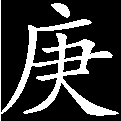
\includegraphics[width=3mm]{../Images/00004}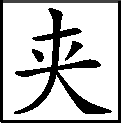
\includegraphics[width=3mm]{../Images/00012}\footnotesize \kaishu 《在园杂{(字)}{[}志{]}》曾有此说。}碧糯五十斛,白糯五十斛,粉粳五十斛,杂色粱谷各五十斛,下用常米一千石,各色干菜一车,外卖粱谷、牲口各项之银共折银二千五百两。外门下孝敬哥儿姐儿顽意:活鹿两对,活白兔四对,黑兔四对,活锦鸡两对,西洋鸭两对。”

贾珍便命带进他来。一时,只见乌进孝进来,只在院内磕头请安。贾珍命人拉他起来,笑说:“你还硬朗。”乌进孝笑回:“托爷的福,还能走得动。”贾珍道:“你儿子也大了,该叫他走走也罢了。”乌进孝笑道:“不瞒爷说,小的们走惯了,不来也闷的慌。他们可不是都愿意来见见天子脚下世面?他们到底年轻,怕路上有闪失,再过几年就可放心了。”贾珍道:“你走了几日?”乌进孝道:“回爷的话,今年雪大,外头都是四五尺深的雪,前日忽然一暖一化,路上竟难走的很,耽搁了几日。虽走了一个月零两日,因日子有限了,怕爷心焦,可不赶着来了。”贾珍道:“我说呢,怎么今儿才来。我才看那单子上,今年你这老货又来打擂台来了。”乌进孝忙进前了两步,回道:“回爷说,今年年成实在不好。从三月下雨起,接接连连直到八月,竟没有一连晴过五日。九月里一场碗大的雹子,方近一千三百里地,连人带房并牲口粮食,打伤了上千上万的,所以才这样。小的并不敢说谎。”贾珍皱眉道:“我算定了你至少也有五千两银子来,这够作什么的!如今你们一共只剩了八九个庄子,今年倒有两处报了旱涝,你们又打擂台,真真是又教别过年了。”乌进孝道:“爷的这地方还算好呢!我兄弟离我那里只一百多里,谁知竟大差了。他现管着那府里八处庄地,比爷这边多着几倍,今年也只这些东西,不过多二三千两银子,也是有饥荒打呢。”贾珍道:“正是呢,我这边都可以,没有什么外项大事,不过是一年的费用。费些我就受用些,我受些委屈就省些。再者年例送人请人,我把脸皮厚些,可省些也就完了。比不得那府里,这几年添了许多花钱的事,一定不可免是要花的,却又不添些银子产业。这一二年倒赔了许多,不和你们要,找谁去!”乌进孝笑道:“那府里如今虽添了事,有去有来,娘娘和万岁爷岂不赏的!”{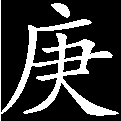
\includegraphics[width=3mm]{../Images/00004}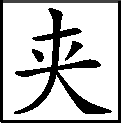
\includegraphics[width=3mm]{../Images/00012}\footnotesize \kaishu 是庄头口中语气。脂砚。}贾珍听了,笑向贾蓉等道:“你们听,他这话可笑不可笑?”贾蓉等忙笑道:“你们山坳海沿子上的人,那里知道这道理。娘娘难道把皇上的库给了我们不成!他心里纵有这心,他也不能作主。岂有不赏之理,按时到节不过是些彩缎古董顽意儿。纵赏银子,不过一百两金子,才值了一千两银子,够一年的什么?这二年那一年不多赔出几千银子来!头一年省亲连盖花园子,你算算那一注共花了多少,就知道了。再两年再一回省亲,只怕就净穷了。”贾珍笑道:“所以他们庄家老实人,外明不知里暗的事。黄柏木作磬槌子------外头体面里头苦。”{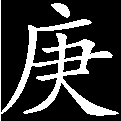
\includegraphics[width=3mm]{../Images/00004}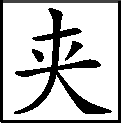
\includegraphics[width=3mm]{../Images/00012}\footnotesize \kaishu 新鲜趣语。}贾蓉又笑向贾珍道:“果真那府里穷了。前儿我听见凤姑娘{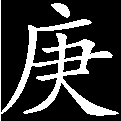
\includegraphics[width=3mm]{../Images/00004}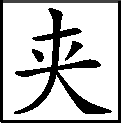
\includegraphics[width=3mm]{../Images/00012}\footnotesize \kaishu 此亦南北互用之文,前注不谬。}和鸳鸯悄悄商议,要偷出老太太的东西去当银子呢。”贾珍笑道:“那又是你凤姑娘的鬼,那里就穷到如此。他必定是见去路太多了,实在赔的狠了,不知又要省那一项的钱,先设此法使人知道,说穷到如此了。我心里却有一个算盘,还不至如此田地。”说着,命人带了乌进孝出去,好生待他,不在话下。

这里贾珍吩咐将方才各物,留出供祖的来,将各样取了些,命贾蓉送过荣府里。然后自己留了家中所用的,馀者派出等例来,一分一分的堆在月台下,命人将族中的子侄唤来与他们。接着荣国府也送了许多供祖之物及与贾珍之物。贾珍看着收拾完备供器,靸着鞋,披着猞猁狲大裘,命人在厅柱下石矶上太阳中铺了一个大狼皮褥子,负暄闲看各子弟们来领取年物。因见贾芹亦来领物,贾珍叫他过来,说道:“你作什么也来了?谁叫你来的?”贾芹垂手回说:“听见大爷这里叫我们领东西,我没等人去就来了。”贾珍道:“我这东西,原是给你那些闲着无事的无进益的小叔叔兄弟们的。那二年你闲着,我也给过你的。你如今在那府里管事,家庙里管和尚道士们,一月又有你的分例外,这些和尚的分例银子都从你手里过,你还来取这个,太也贪了!你自己瞧瞧,你穿的像个手里使钱办事的?先前说你没进益,如今又怎么了?比先倒不像了。”贾芹道:“我家里原人口多,费用大。”贾珍冷笑道:“你还支吾我。你在家庙里干的事,打量我不知道呢。你到了那里自然是爷了,没人敢违拗你。你手里又有了钱,离着我们又远,你就为王称霸起来,夜夜招聚匪类赌钱,{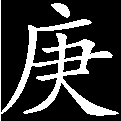
\includegraphics[width=3mm]{../Images/00004}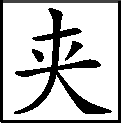
\includegraphics[width=3mm]{../Images/00012}\footnotesize \kaishu 这一回文字断不可少。}养老婆小子。这会子花的这个形象,你还敢领东西来?领不成东西,领一顿驮水棍去才罢。等过了年,我必和你琏二叔说,换回你来。”贾芹红了脸,不敢答应。人回:“北府水王爷送了字联、荷包来了。”贾珍听说,忙命贾蓉出去款待,“只说我不在家。”贾蓉去了,这里贾珍看着领完东西,回房与尤氏吃毕晚饭,一宿无话。至次日,更比往日忙,都不必细说。

已到了腊月二十九日了,各色齐备,两府中都换了门神、联对、挂牌,新油了桃符,焕然一新。宁国府从大门、仪门、大厅、暖阁、内厅、内三门、内仪门并内塞门,直到正堂,一路正门大开,两边阶下一色朱红大高照,点的两条金龙一般。次日,由贾母有诰封者,皆按品级着朝服,先坐八人大轿,带领着众人进宫朝贺,行礼领宴毕回来,便到宁国府暖阁下轿。诸子弟有未随入朝者,皆在宁府门前排班伺候,然后引入宗祠。且说宝琴是初次,一面细细留神打量这宗祠,原来宁府西边另一个院子,黑油栅栏内五间大门,上悬一块匾,写着是“贾氏宗祠”四个字,旁书“衍圣公孔继宗书”。两旁有一副长联,写道是:

肝脑涂地,兆姓赖保育之恩;

功名贯天,百代仰蒸尝之盛。

亦衍圣公所书。进入院中,白石甬路,两边皆是苍松翠柏。月台上设着青绿古铜鼎彝等器。抱厦前上面悬一九龙金匾,写道是:“星辉辅弼”。乃先皇御笔。两边一副对联,写道是:

勋业有光昭日月,功名无间及儿孙。

亦是御笔。五间正殿前悬一闹龙填青匾,写道是:“慎终追远”。旁边一副对联,写道是:

已后儿孙承福德,至今黎庶念荣宁。

俱是御笔。里边香烛辉煌,锦帐绣幕,虽列着神主,却看不真切。只见贾府人分昭穆排班立定:贾敬主祭,贾赦陪祭,贾珍献爵,贾琏贾琮献帛,宝玉捧香,贾菖贾菱展拜毯,守焚池。青衣乐奏,三献爵,拜兴毕,焚帛奠酒。礼毕,乐止,退出。众人围随贾母至正堂上,影前锦幔高挂,彩屏张护,香烛辉煌。上面正居中悬着宁荣二祖遗像,皆是披蟒腰玉;两边还有几轴列祖遗影。贾荇贾芷等从内仪门挨次列站,直到正堂廊下。槛外方是贾敬贾赦,槛内是各女眷。众家人小厮皆在仪门之外。每一道菜至,传至仪门,贾荇贾芷等便接了,按次传至阶上贾敬手中。贾蓉系长房长孙,独他随女眷在槛内,每贾敬捧菜至,传于贾蓉,贾蓉便传于他妻子,又传于凤姐尤氏诸人,直传至供桌前,方传于王夫人。王夫人传于贾母,贾母方捧放在桌上。邢夫人在供桌之西,东向立,同贾母供放。直至将菜饭汤点酒茶传完,贾蓉方退出下阶,归入贾芹阶位之首。

凡从文旁之名者,贾敬为首;下则从玉者,贾珍为首;再下从草头者,贾蓉为首;左昭右穆,男东女西;俟贾母拈香下拜,众人方一齐跪下,将五间大厅,三间抱厦,内外廊檐,阶上阶下两丹墀内,花团锦簇,塞的无一隙空地。鸦雀无闻,只听铿锵叮当,金铃玉佩微微摇曳之声,并起跪靴履飒沓之响。一时礼毕,贾敬贾赦等便忙退出,至荣府专候与贾母行礼。

尤氏上房早已袭地铺满红毡,当地放着象鼻三足鳅沿鎏金珐琅大火盆,正面炕上铺新猩红毡,设着大红彩绣云龙捧寿的靠背引枕,外另有黑狐皮的袱子搭在上面,大白狐皮坐褥,请贾母上去坐了。两边又铺皮褥,让贾母一辈的两三个妯娌坐了。这边横头排插之后小炕上,也铺了皮褥,让邢夫人等坐了。地下两面相对十二张雕漆椅上,都是一色灰鼠椅搭小褥,每一张椅下一个大铜脚炉,让宝琴等姊妹坐了。尤氏用茶盘亲捧茶与贾母,蓉妻捧与众老祖母,然后尤氏又捧与邢夫人等,蓉妻又捧与众姊妹。凤姐李纨等只在地下伺候。茶毕,邢夫人等便先起身来侍贾母。贾母吃茶,与老妯娌闲话了两三句,便命看轿,凤姐儿忙上去挽起来。尤氏笑回说:“已经预备下老太太的晚饭。每年都不肯赏些体面用过晚饭过去,果然我们就不及凤丫头不成?”凤姐儿搀着贾母笑道:“老祖宗快走,咱们家去吃去,别理他。”贾母笑道:“你这里供着祖宗,忙的什么似的,那里还搁得住闹。况且每年我不吃,你们也要送去的。不如还送了来,我吃不了留着明儿再吃,岂不多吃些。”说的众人都笑了。又吩咐他:”好生派妥当人夜里看香火,不是大意得的。”尤氏答应了。一面走出来至暖阁前上了轿。尤氏等闪过屏风,小厮们才领轿夫,请了轿出大门。尤氏亦随邢夫人等同至荣府。

这里轿出大门,这一条街上,东一边合面设列着宁国府的仪仗执事乐器,西一边合面设列着荣国府的仪仗执事乐器,来往行人皆屏退不从此过。一时来至荣府,也是大门正厅直开到底。如今便不在暖阁下轿了,过了大厅,便转弯向西,至贾母这边正厅上下轿。众人围随同至贾母正室之中,亦是锦裀绣屏,焕然一新。当地火盆内焚着松柏香、百合草。贾母归了座,老嬷嬷来回:“老太太们来行礼。”贾母忙又起身要迎,只见两三个老妯娌已进来了。大家挽手,笑了一回,让了一回。吃茶去后,贾母只送至内仪门便回来,归正坐。贾敬贾赦等领诸子弟进来。贾母笑道:“一年价难为你们,不行礼罢。”一面说着,一面男一起,女一起,一起一起俱行过了礼。左右两旁设下交椅,然后又按长幼挨次归坐受礼。两府男妇小厮丫鬟亦按差役上中下行礼毕,散押岁钱、荷包、金银锞,摆上合欢宴来。男东女西归坐,献屠苏酒、合欢汤、吉祥果、如意糕毕,贾母起身进内间更衣,众人方各散出。那晚各处佛堂灶王前焚香上供,王夫人正房院内设着天地纸马香供,大观园正门上也挑着大明角灯,两溜高照,各处皆有路灯。上下人等,皆打扮的花团锦簇,一夜人声嘈杂,语笑喧阗,爆竹起火,络绎不绝。

至次日五鼓,贾母等又按品大妆,摆全副执事进宫朝贺,兼祝元春千秋。领宴回来,又至宁府祭过列祖,方回来受礼毕,便换衣歇息。所有贺节来的亲友一概不会,只和薛姨妈李婶二人说话取便,或者同宝玉、宝琴、钗、玉等姊妹赶围棋抹牌作戏。王夫人与凤姐是天天忙着请人吃年酒,那边厅上院内皆是戏酒,亲友络绎不绝,一连忙了七八日才完了。早又元宵将近,宁荣二府皆张灯结彩。十一日是贾赦请贾母等,次日贾珍又请,贾母皆去随便领了半日。王夫人和凤姐儿连日被人请去吃年酒,不能胜记。

至十五日之夕,贾母便在大花厅上命摆几席酒,定一班小戏,满挂各色佳灯,带领荣宁二府各子侄孙男孙媳等家宴。贾敬素不茹酒,也不去请他,于后十七日祖祀已完,他便仍出城去修养。便这几日在家内,亦是静室默处,一概无听无闻,不在话下。贾赦略领了贾母之赐,也便告辞而去。贾母知他在此彼此不便,也就随他去了。贾赦自到家中与众门客赏灯吃酒,自然是笙歌聒耳,锦绣盈眸,其取便快乐另与这边不同的。{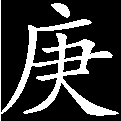
\includegraphics[width=3mm]{../Images/00004}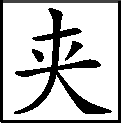
\includegraphics[width=3mm]{../Images/00012}\footnotesize \kaishu 又交代一个。}

这边贾母花厅之上共摆了十来席。每一席旁边设一几,几上设炉瓶三事,焚着御赐百合宫香。又有八寸来长四五寸宽二三寸高的点着山石布满青苔的小盆景,俱是新鲜花卉。又有小洋漆茶盘,内放着旧窑茶杯并十锦小茶吊,里面泡着上等名茶。一色皆是紫檀透雕,嵌着大红纱透绣花卉并草字诗词的璎珞。原来绣这璎珞的也是个姑苏女子,名唤慧娘。因他亦是书香宦门之家,他原精于书画,不过偶然绣一两件针线作耍,并非市卖之物。凡这屏上所绣之花卉,皆仿的是唐、宋、元、明各名家的折枝花卉,故其格式配色皆从雅,本来非一味浓艳匠工可比。每一枝花侧皆用古人题此花之旧句,或诗词歌赋不一,皆用黑绒绣出草字来,且字迹勾踢、转折、轻重、连断皆与笔草无异,亦不比市绣字迹板强可恨。他不仗此技获利,所以天下虽知,得者甚少,凡世宦富贵之家,无此物者甚多,当今便称为“慧绣”。竟有世俗射利者,近日仿其针迹,愚人获利。偏这慧娘命夭,十八岁便死了,如今竟不能再得一件的了。凡所有之家,纵有一两件,皆珍藏不用。有那一干翰林文魔先生们,因深惜“慧绣”之佳,便说这“绣”字不能尽其妙,这样笔迹说一“绣”字,反似乎唐突了,便大家商议了,将“绣”字便隐去,换了一个“纹”字,所以如今都称为“慧纹”。若有一件真“慧纹”之物,价则无限。贾府之荣,也只有两三件,上年将那两件已进了上,目下只剩这一副璎珞,一共十六扇,贾母爱如珍宝,不入在请客各色陈设之内,只留在自己这边,高兴摆酒时赏玩。又有各色旧窑小瓶中都点缀着“岁寒三友”“玉堂富贵”等鲜花草。

上面两席是李婶薛姨妈二位。贾母于东边设一透雕夔龙护屏矮足短榻,靠背引枕皮褥俱全。榻之上一头又设一个极轻巧洋漆描金小几,几上放着茶吊、茶碗、漱盂、洋巾之类,又有一个眼镜匣子。贾母歪在榻上,与众人说笑一回,又自取眼镜向戏台上照一回,又向薛姨妈李婶笑说:“恕我老了,骨头疼,放肆,容我歪着相陪罢。”因又命琥珀坐在榻上,拿着美人拳捶腿。

榻下并不摆席面,只有一张高几,却设着璎珞花瓶香炉等物。外另设一精致小高桌,设着酒杯匙箸,将自己这一席设于榻旁,命宝琴、湘云、黛玉、宝玉四人坐着。每一馔一果来,先捧与贾母看了,喜则留在小桌上尝一尝,仍撤了放在他四人席上,只算他四人是跟着贾母坐。故下面方是邢夫人王夫人之位,再下便是尤氏、李纨、凤姐、贾蓉之妻。西边一路便是宝钗、李纹、李绮、岫烟、迎春姊妹等。两边大梁上,挂着一对联三聚五玻璃芙蓉彩穗灯。每一席前竖一柄漆干倒垂荷叶,叶上有烛信插着彩烛。这荷叶乃是錾珐琅的,活信可以扭转,如今皆将荷叶扭转向外,将灯影逼住全向外照,看戏分外真切。窗格门户一齐摘下,全挂彩穗各种宫灯。廊檐内外及两边游廊罩棚,将各色羊角、玻璃、戳纱、料丝、或绣、或画、或堆、或抠、或绢、或纸诸灯挂满。

廊上几席,便是贾珍、贾琏、贾环、贾琮、贾蓉、贾芹、贾芸、贾菱、贾菖等。贾母也曾差人去请众族中男女,奈他们或有年迈懒于热闹的;或有家内没有人不便来的;或有疾病淹缠,欲来竟不能来的;或有一等妒富愧贫不来的;甚至于有一等憎畏凤姐之为人而赌气不来的;或有羞手羞脚,不惯见人,不敢来的:因此族众虽多,女客来者只不过贾菌之母娄氏带了贾菌来了,男子只有贾芹、贾芸、贾菖、贾菱四个现是在凤姐麾下办事的来了。当下人虽不全,在家庭间小宴中,数来也算是热闹的了。

当下又有林之孝之妻带了六个媳妇,抬了三张炕桌,每一张上搭着一条红毡,毡上放着选净一般大新出局的铜钱,用大红彩绳串着,每二人搭一张,共三张。林之孝家的指示将那两张摆至薛姨妈李婶的席下,将一张送至贾母榻下来。贾母便说:“放在当地罢。”这媳妇们都素知规矩的,放下桌子,一并将钱都打开,将彩绳抽去,散堆在桌上。

正唱《西楼·楼会》这出将终,于叔夜因赌气去了,那文豹便发科诨道:“你赌气去了,恰好今日正月十五,荣国府中老祖宗家宴,待我骑了这马,赶进去讨些果子吃是要紧的。”说毕,引的贾母等都笑了。薛姨妈等都说:“好个鬼头孩子,可怜见的。”凤姐便说:“这孩子才九岁了。”贾母笑说:“难为他说的巧。”便说了一个“赏”字。早有三个媳妇已经手下预备下小簸箩,听见一个“赏”字,走上去向桌上的散钱堆内,每人便撮了一簸箩,走出来向戏台说:“老祖宗、姨太太、亲家太太赏文豹买果子吃的!”说着,向台上便一撒,只听豁啷啷满台的钱响。

贾珍贾琏已命小厮们抬了大簸箩的钱来,暗暗的预备在那里。听见贾母一赏,要知端的------

{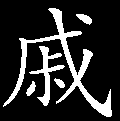
\includegraphics[width=3mm]{../Images/00005}  \kaishu 总评:叙元宵一宴,却不叙酒何以清,菜何以馨,客何以盛,令何以行。先于香茗古玩上渲染,几榻坐次上铺叙,隐隐为下回张本,有无限含蓄,超迈獭祭者百倍。}

{前半整饬,后半疏落,浓淡相间。祭宗祠在宁府,开夜宴在荣府,分叙不犯手,是作者胸有成竹处。}
